\documentclass[journal,12pt,twocolumn]{IEEEtran}
%
\usepackage{setspace}
\usepackage{gensymb}
\usepackage{xcolor}
\usepackage{caption}
%\usepackage{subcaption}
%\doublespacing
\singlespacing

%\usepackage{graphicx}
%\usepackage{amssymb}
%\usepackage{relsize}
\usepackage[cmex10]{amsmath}
\usepackage{mathtools}
%\usepackage{amsthm}
%\interdisplaylinepenalty=2500
%\savesymbol{iint}
%\usepackage{txfonts}
%\restoresymbol{TXF}{iint}
%\usepackage{wasysym}
\usepackage{hyperref}
\usepackage{amsthm}
\usepackage{mathrsfs}
\usepackage{txfonts}
\usepackage{stfloats}
\usepackage{cite}
\usepackage{cases}
\usepackage{subfig}
%\usepackage{xtab}
\usepackage{longtable}
\usepackage{multirow}
%\usepackage{algorithm}
%\usepackage{algpseudocode}
%\usepackage{enumerate}
\usepackage{enumitem}
\usepackage{mathtools}
%\usepackage{iithtlc}
%\usepackage[framemethod=tikz]{mdframed}
\usepackage{listings}
\usepackage{scalerel}
\usepackage{stackengine}
\usepackage{xcolor}
\newcommand\showdiv[1]{\overline{\smash{\hstretch{.5}{)}\mkern-3.2mu\hstretch{.5}{)}}#1}}
\usepackage{polynom}
%\usepackage{stmaryrd}
\let\vec\mathbf

%\usepackage{wasysym}
%\newcounter{MYtempeqncnt}
\DeclareMathOperator*{\Res}{Res}
%\renewcommand{\baselinestretch}{2}
\renewcommand\thesection{\arabic{section}}
\renewcommand\thesubsection{\thesection.\arabic{subsection}}
\renewcommand\thesubsubsection{\thesubsection.\arabic{subsubsection}}

\renewcommand\thesectiondis{\arabic{section}}
\renewcommand\thesubsectiondis{\thesectiondis.\arabic{subsection}}
\renewcommand\thesubsubsectiondis{\thesubsectiondis.\arabic{subsubsection}}

%\renewcommand{\labelenumi}{\textbf{\theenumi}}
%\renewcommand{\theenumi}{P.\arabic{enumi}}

% correct bad hyphenation here
\hyphenation{op-tical net-works semi-conduc-tor}

\lstset{
	language=Python,
	frame=single, 
	breaklines=true,
	columns=fullflexible
}



\begin{document}
	%
	
	\theoremstyle{definition}
	\newtheorem{theorem}{Theorem}[section]
	\newtheorem{problem}{Problem}
	\newtheorem{proposition}{Proposition}[section]
	\newtheorem{lemma}{Lemma}[section]
	\newtheorem{corollary}[theorem]{Corollary}
	\newtheorem{example}{Example}[section]
	\newtheorem{definition}{Definition}[section]
	%\newtheorem{algorithm}{Algorithm}[section]
	%\newtheorem{cor}{Corollary}
	\newcommand{\BEQA}{\begin{eqnarray}}
		\newcommand{\EEQA}{\end{eqnarray}}
	\newcommand{\define}{\stackrel{\triangle}{=}}
	\newcommand{\myvec}[1]{\ensuremath{\begin{pmatrix}#1\end{pmatrix}}}
	\newcommand{\mydet}[1]{\ensuremath{\begin{vmatrix}#1\end{vmatrix}}}
	
	
	\bibliographystyle{IEEEtran}
	%\bibliographystyle{ieeetr}
	
	\providecommand{\nCr}[2]{\,^{#1}C_{#2}} % nCr
	\providecommand{\nPr}[2]{\,^{#1}P_{#2}} % nPr
	\providecommand{\mbf}{\mathbf}
	\providecommand{\pr}[1]{\ensuremath{\Pr\left(#1\right)}}
	\providecommand{\qfunc}[1]{\ensuremath{Q\left(#1\right)}}
	\providecommand{\sbrak}[1]{\ensuremath{{}\left[#1\right]}}
	\providecommand{\lsbrak}[1]{\ensuremath{{}\left[#1\right.}}
	\providecommand{\rsbrak}[1]{\ensuremath{{}\left.#1\right]}}
	\providecommand{\brak}[1]{\ensuremath{\left(#1\right)}}
	\providecommand{\lbrak}[1]{\ensuremath{\left(#1\right.}}
	\providecommand{\rbrak}[1]{\ensuremath{\left.#1\right)}}
	\providecommand{\cbrak}[1]{\ensuremath{\left\{#1\right\}}}
	\providecommand{\lcbrak}[1]{\ensuremath{\left\{#1\right.}}
	\providecommand{\rcbrak}[1]{\ensuremath{\left.#1\right\}}}
	\theoremstyle{remark}
	\newtheorem{rem}{Remark}
	\newcommand{\sgn}{\mathop{\mathrm{sgn}}}
	
	\providecommand{\abs}[1]{\left\vert#1\right\vert}
	\providecommand{\res}[1]{\Res\displaylimits_{#1}} 
	\providecommand{\norm}[1]{\lVert#1\rVert}
	\providecommand{\mtx}[1]{\mathbf{#1}}
	\providecommand{\mean}[1]{E\left[ #1 \right]}
	\providecommand{\fourier}{\overset{\mathcal{F}}{ \rightleftharpoons}}
	\providecommand{\ztrans}{\overset{\mathcal{Z}}{ \rightleftharpoons}}
	
	%\providecommand{\hilbert}{\overset{\mathcal{H}}{ \rightleftharpoons}}
	\providecommand{\system}{\overset{\mathcal{H}}{ \longleftrightarrow}}
	%\newcommand{\solution}[2]{\textbf{Solution:}{#1}}
	\newcommand{\solution}{\noindent \textbf{Solution: }}
	\providecommand{\dec}[2]{\ensuremath{\overset{#1}{\underset{#2}{\gtrless}}}}
	\numberwithin{equation}{section}
	%\numberwithin{equation}{subsection}
	%\numberwithin{problem}{subsection}
	%\numberwithin{definition}{subsection}
	\makeatletter
	\@addtoreset{figure}{problem}
	\makeatother
	
	\let\StandardTheFigure\thefigure
	%\renewcommand{\thefigure}{\theproblem.\arabic{figure}}
	\renewcommand{\thefigure}{\theproblem}
	
	
	%\numberwithin{figure}{subsection}
	
	\def\putbox#1#2#3{\makebox[0in][l]{\makebox[#1][l]{}\raisebox{\baselineskip}[0in][0in]{\raisebox{#2}[0in][0in]{#3}}}}
	\def\rightbox#1{\makebox[0in][r]{#1}}
	\def\centbox#1{\makebox[0in]{#1}}
	\def\topbox#1{\raisebox{-\baselineskip}[0in][0in]{#1}}
	\def\midbox#1{\raisebox{-0.5\baselineskip}[0in][0in]{#1}}
	
	\vspace{5cm}
	
	\title{EE 3900 - Assignment 3}
	
	\author{VIBHAVASU}
	
	\maketitle
	

\vspace{5cm}
\section{Oppenhiem 2.29 a}

Given Discrete time signal:\\
\begin{align}
x[n] = \begin{cases}
	1	& $if $-1 \leq x \leq 3\\
	\dfrac{1}{2} & $if $ x = 4\\
	0 & $everywhere else$
\end{cases}
\end{align}
\newline
It is plotted in the following figure:
\begin{figure}[!ht]
	\begin{center}
		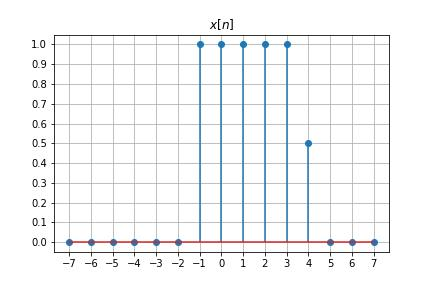
\includegraphics[width=\columnwidth]{./figs/xn.jpg}
	\end{center}
	\caption{$x[n]$}
	\label{fig:x[n]}	
\end{figure}
\section*{Question: Find and plot $x[n-2]$}
\section{\solution}
\begin{align}
	1	& $ if $1 \leq x \leq 5\\
	\dfrac{1}{2} & $ if $ x = 6\\
	0 & $everywhere else$
\end{cases}
\end{align}	
$x[n-2]$ is plotted in the following figure
\begin{figure}[!ht]
	\begin{center}
		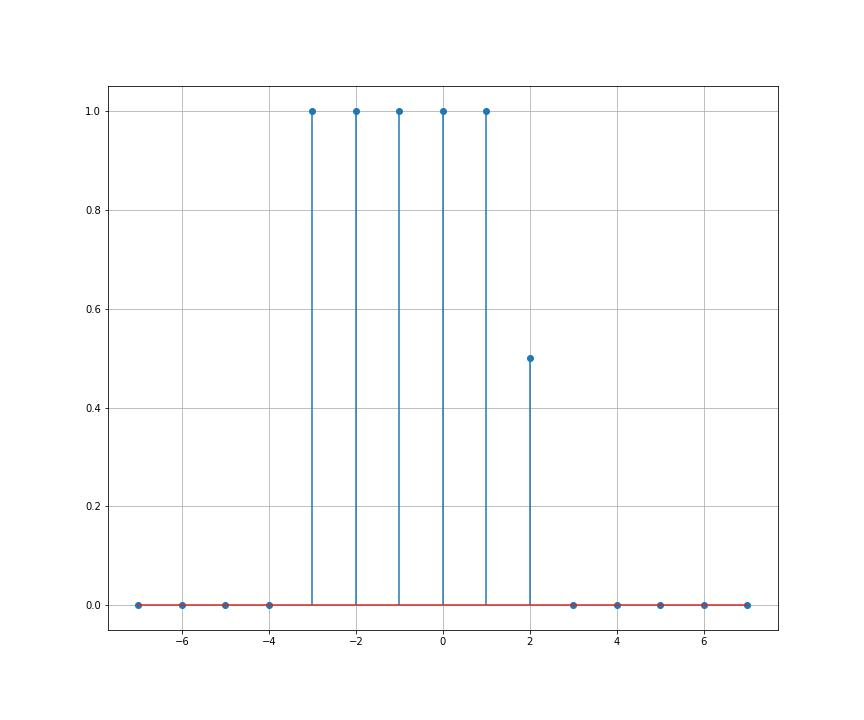
\includegraphics[width=\columnwidth]{./figs/xn2.jpg}
	\end{center}
	\caption{$x[n - 2]$}
	\label{fig:x[n-2]}	
\end{figure}

\vspace{6cm}

The code used for this exercise can found at:\\


\begin{lstlisting}
wget https://raw.githubusercontent.com/gadepall/EE1310/master/Assignment 3/a3.ipynb
\end{lstlisting}

\newpage
For $i^{th}$ neutrino and $j^{th}$ pulsar:
\begin{align*}
	S_{ij} = \frac{1}{2\pi\sigma_i^2}e^{-(|\theta_i-\theta_j|)^2/2\sigma_i^2}\\
	S_i = \sum_{j = 0}^{p}\dfrac{S_{ij}}{ns[j]}
\end{align*}
where ns[j] is the no.of events associated with $j^{th}$ source/pulsar

\begin{align*}
	B_i = \dfrac{\text{total no of neutrino events within $ \delta \pm 3$ of $\nu_i$}}{2\pi(\sin(\delta + 3) - \sin(\delta + 3))}
\end{align*}


\end{document}